\section{\large Аналитическая часть}

В данном разделе проводится анализ предметной области, анализ паттерна \textit{thread pool}, асинхронной блокирующей модели ввода-вывда и системного вызова \textit{pselect}, а также протокол HTTP и формализация требований к разрабатываемой программе.

\subsection{Статическая информация}

Статическая информация --- информация, которая редко меняется с течением времени. В данной работе под статической информацией будем подразумевать файлы определённых форматоов, которые, предположительно, редко меняются с течением времени. 

Согласно поставленной задаче, разрабатываемый сервер разадчи статической инфоормации должен предоставлять доступ к файлам следующих форматов:
\begin{enumerate}[label=\arabic*)]
	\item файлы HTML (имеющие расширение .html), содержащие гипертекстовые документы;
	\item скрипты JS (имеющие расширение .js);
	\item файлы стилей CSS (имеющие расширение .css) ;
	\item файлы изображений форматов PNG и JPEG (имеющие расширения .png и .jpeg или .jpg  соответственно);
	\item файлы SWF для векторной анимации (имеющие расширение .swf);
	\item файлы GIF, содержащие графические изображения или анимации (имеющие расширение .gif).
\end{enumerate}

Также необходимо учесть, что рассмотренные файлы могут иметь размер до нескольких сотен мегабайт, и передача таких файлов должна осуществляться корректно.

\subsection{Существующие решения}

Поскольку проблема раздачи статической информации возникла вместе с появлением интернета, к 2023 году существует набор готвых решений, как универсальных, так и направленных на соответствие определённым технологиям. 

NGINX (от англ. \textit{Engine X}) --- веб-сервер и прокси-сервер, работающий как на Unix-подобных системах, так и на системах Miscrosoft Windows (с версии 0.7.72). Разработан в 2004 году российским программистом Игорем Сысоевым, выпускником МГТУ~им.~Н.~Э.~Баумана. NGINX позиционируется производителем как простой, быстрый и надёжный сервер, использование корого целесообразно в том числе для раздачи статической информации. Помимо раздачи статической информации, NGINX предоставляет возможности кэширования запросов, сжатия при помощи технологии gzip, балансировки нагрузки между серверами, а также многие другие функции \cite{nginx}. По данным Netcrafts, к ноябрю 2023 года NGINX используется для поддержки 249 миллионов сайтов, что составляет большую часть (22.83\%) опрошенных сайтов \cite{nginx-popular}.

Apache (от англ. \textit{a patchy server}) --- ближайший конкурент NGINX в области веб-серверов, является веб-сервером с открытым исходным кодом, поддержкивает такие операционные системы, как Linux, BSD, macOS и Microsoft Windows. C апреля 1996 года и по июль 2016 года являлся самым популярным веб-сервером в мире, поскольку с момента появления интернета являлся самым надёжным сервером, сейчас же используется 22.74\% сайтов, лишь немнго уступая NGINX \cite{nginx-popular}.

Cloudflare --- американская компания, предоставляющая услуги по раздаче статической информации, защите от атак, предоставлению серверов DNS и проксированию сайтов. Услугами данной компании пользуются 10.62\% опрошенных (115 миллионов сайтов), при этом раздача статической информации не стоит у компании на первом месте, отдаётся приоритет защите от DDoS атак: так, в 2014 году Cloudflare выдержала атаку мощностью 400 Гбит / c.


\subsection{Паттерн пула потоков}

Пул потоков (англ. \textit{thread pool}) --- архитектурный паттерн, предназначенный для многопоточной обработи информации \cite{thread-pool}. В то время как создавать новый поток под новый запрос является неэффективно, предлагается создать набор потоков (пул) определённй величины, и поддерживать его на протяжении работы программы. Когда на сервер приходит запрос, предлагается использовать свободный поток из пула потоков. В данном потоке будет произведена обработка пришедшего запроса, после чего поток будет возвращён в пул потоков, готовый к обработке дальнейших запросов. 

Исследования \cite{thread-pool} показали, что использование пула потоков может значительно улучшить производительность системы и уменьшить время обработки запросов. Тем не менее, существуют следующие проблемы, возникающие при использовании пула потоков:

\begin{itemize}[leftmargin=1.6\parindent]
	\item[---] определение числа потоков (размера пула);
	\item[---] контроль целостности очереди и предотвращения обработки одного запроса двумя потоками;
	\item[---] оптимальное использование вычислительных ресурсов и предотвращение "простаивания" потоков.
\end{itemize}

В данной работе предлагается оставить возможность указывать количество потоков при запуске сервера. Это позволит использовать разработанную программу наиболее гибко. 

Последние две проблемы предлагается решить при помощи средств взаимоисключения (например, mutex-ов), а также использования каждым потом своего сокета, обеспечив неблокирующий ввод-вывод посредством сокетов.
На рисунке \ref{fig:threadpool} представлена концептуальная модель пула потоков: очередь запросов, ожидающих обработку, пул потоков и обработанные запросы.

\begin{figure}[h!]
	\centering
	\captionsetup{justification=centering}
	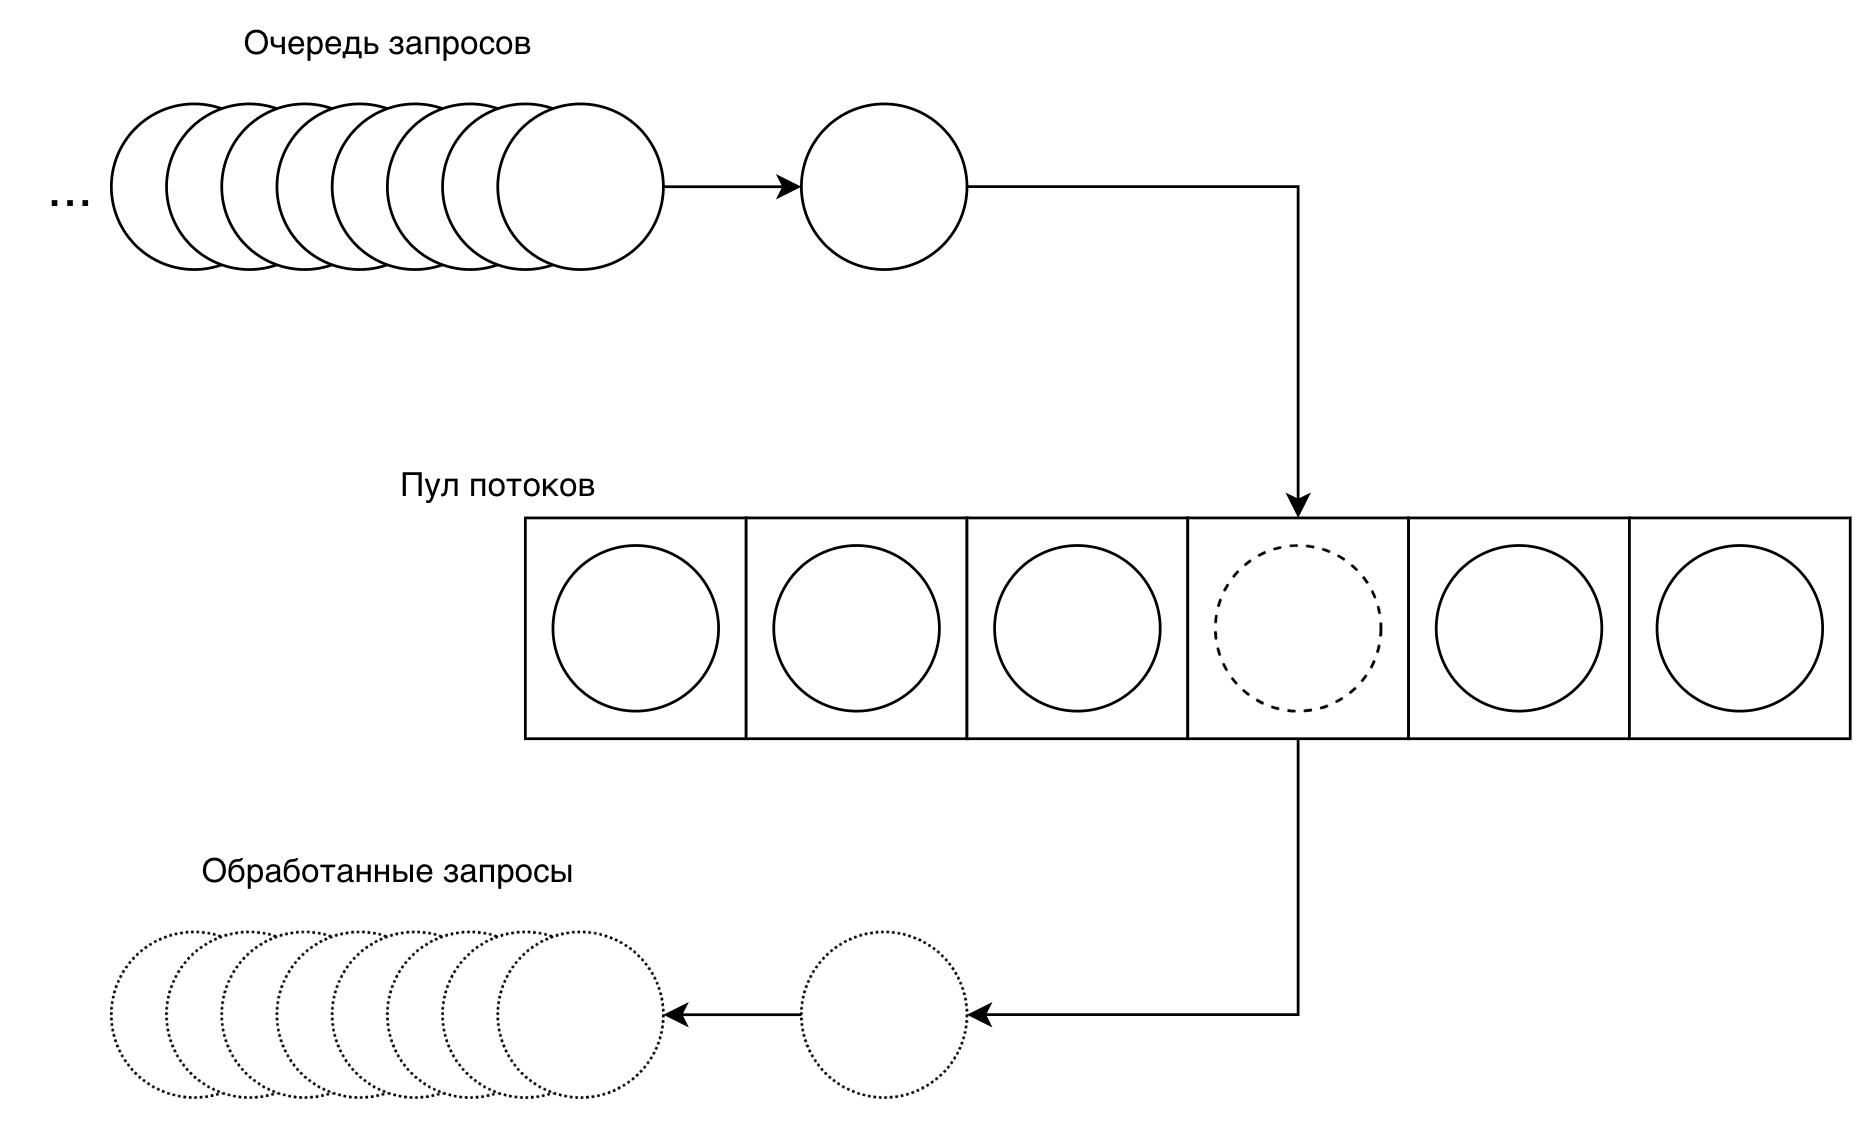
\includegraphics[width=150mm]{img/threadpool.png}
	\caption{Концептуальная модель пула потоков}
	\label{fig:threadpool}
\end{figure}

\subsection{Асинхронный блокирующий ввод-вывод}

Прежде, чем перейти к описанию системного вызова \textit{pselect}, рассмотрим модель асинхронного блокирующего ввоода-вывода, в котой этот вызов используется.

Модель асинхронного блокирующего ввода-вывода основана на опросе набора источников ввода-вывода на предмет готовности. Блокировка происходит на моменте опроса: главный процесс блокируется в ожидании готовности соединения. Как только соединение установлено, можно осуществлять передачу и дальнейшую обработку данных. Асинхронным данный метод называется потому, что возможен одновременный опрос нескольких источников ввода-вывода и блокировка лишь до того момента, когда первый из источников сообщит о готовности.

На рисунке \ref{fig:select} представлена модель асинхронного блокирующего ввода-вывода с ипользованием select: запрос  на чтение, блокировка в ожидании результата чтения, передача даннных из пространства ядра в пространство пользователя.

\begin{figure}[h!]
	\centering
	\captionsetup{justification=centering}
	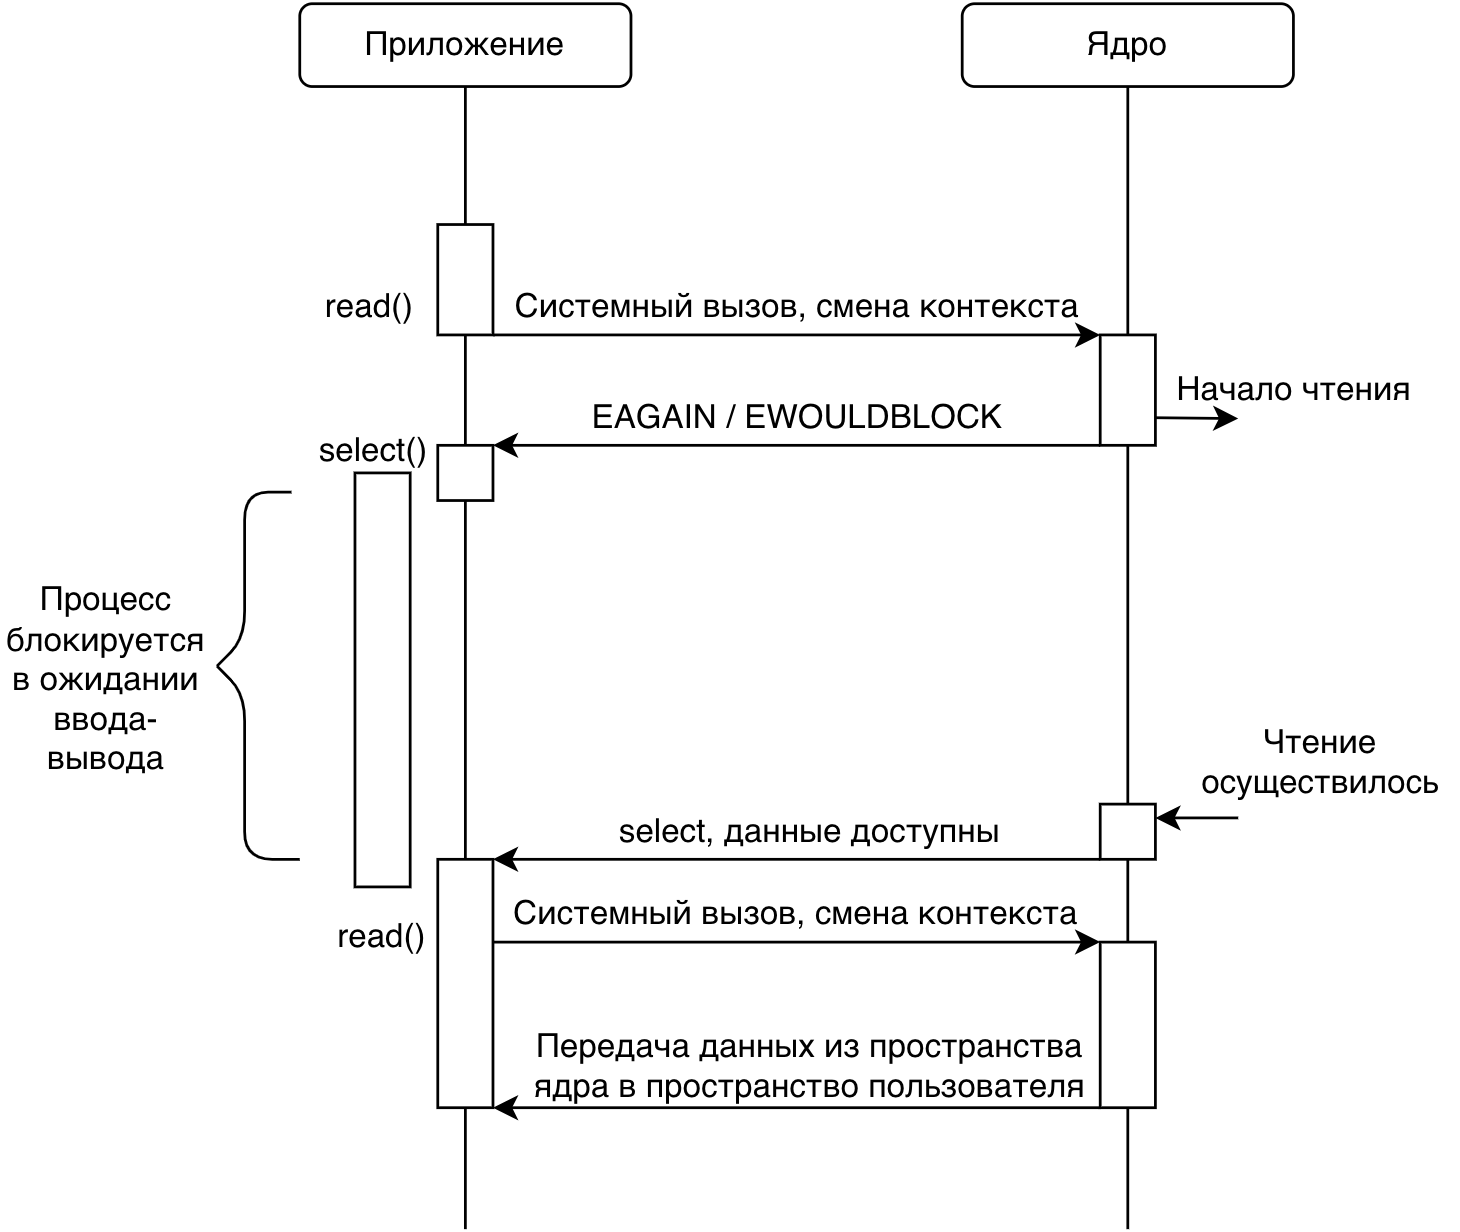
\includegraphics[width=150mm]{img/select.png}
	\caption{Модель асинхронного блокирующего ввода-вывода с ипользованием select}
	\label{fig:select}
\end{figure}



\subsection{Системный вызов pselect}

Системный вызов \textit{pselect} --- функция, существующая в Unix-подобных и POSIX системах и предназначенная для опроса файловых дескрипторов открытых каналов ввода-вывода. Подключение данной функции происходит при помощи заголовочного файла sys/select.h на языке программирования Си.

Функция pselect принимает на вход 6 аргументов: 

\begin{enumerate}[label=\arabic*)]
	\item nfds, число типа int, значение котого вычисляется как $n + 1$, где $n$ --- максимальное значение файлового дескриптора из наборов файловых дескрипторов, опрос которых осуществляется;
	\item readfds, набор файловых дескрипторов типа fd\_set, предназначенных для опроса на предмет чтения из них;
	\item writefds, набор файловых дескрипторов типа fd\_set, предназначенных для опроса на предмет записи в них;
	\item exceptfds, набор файловых дескрипторов типа fd\_set, предназначенных для опроса на предмет появления исключительных ситуаций;
	\item timeout, структура типа struct timespec (содержит миллисекунды и наносекунды), определяет максимальный интервал времени, в течение которого будет осуществлено ожидание;
	\item sigmask, маска типа sigset\_t сигналов, позволяющая изменить маску сигналов на время работы функции select.
\end{enumerate}

Возвращает функция количество файловых дескрипторов, готовых к вводу-выводу, 0 в случае, если за интервал времени timeout таких дескрипторов нет и -1 в случае ошибки.

При использовании в разрабатываемой программе необходимыми будут лишь параметры nfds, readfds и timeout, поскольку при раздаче статической информации требуется чтение с диска в определённый промежуток времени, а не запись на диск или мониторинг исключительных ситуаций на сокетах.

\subsection{HTTP}

HTTP (англ. \textit{Hypertext Transfer Protocol}) --- протокол прикладного уровня OSI ISO, изначально предназначенный для передачи гипертекстовых документов и сейчас являющийся универсальным средством взаимодействия между узлами в интернете. 

HTTP сообщение состоит из трёх частей: стартовой строки, определяющей тип соообщения, заголовков, характеризующих тело сообщения, параметры передачи и прочие сведения,  а также тела сообщения.

Одним из обязательных заголовков в HTTP сообщении является метод запроса: OPTIONS, GET, HEAD, PUT, POST, PATCH, DELETE, TRACE или CONNECT. В данной работе будут рассмотрены лишь два метода: GET и HEAD, поскольку именно они имеют смысл при реализации сервера раздачи статической инфрмации. 

Метод GET используется для запроса содержимого указанного ресурса. Запросы GET считаются идемпотентными, т.~е. результат запроса всегда будет одним и тем же в случае статической информации. В тело запроса при этом отсутствует, а в теле ответа будет находиться содержимое запрошенного ресурса, в случае разрабатываемого сервера --- содержимое запрошенного файла.

Метод HEAD аналогичен методу GET за исключением того, что в ответе HEAD отсутствует тело сообщения. Обычно HEAD-запросы применяются для извлечения метаданных или проверки существования ресурса.

Ещё один заголовок, который необходимо рассмотреть для правильной передачи данных, это Content-Type. Он предназначен для описания типа передаваемых данных для правильной интерпретации на стороне получателя. Для каждого из рассмотренных выше типов значение заколовка будет своим:

\begin{enumerate}[label=\arabic*)]
	\item файлы HTML --- text/html
	\item скрипты JS --- text/javascript;
	\item файлы стилей CSS --- text/css;
	\item файлы изображений форматов PNG и JPEG --- image/png и image/jpeg;
	\item файлы SWF для векторной анимации --- application/x-shockwave-flash;
	\item файлы GIF --- image/gif.
\end{enumerate}

\subsection{Формализация требований к разрабатываемой программе}

На основе рассмотренной выше информации и задания к работе разрабатываемая программа должна соответстовать следующим требваниям:
\begin{enumerate}[label=\arabic*)]
	\item поддержка запросов GET и HEAD (поддержка статусов 200, 403, 404);
	\item ответ на неподдерживаемые запросы статусом 405;
	\item выставление content type в зависимости от типа файла (поддержка .html, .css, .js, .png, .jpg, .jpeg, .swf, .gif);
	\item корректная передача файлов размером в 100мб;
	\item сервер по умолчанию должен возвращать html-страницу на выбранную тему с css-стилем;
	\item учесть минимальные требования к безопасности статик-серверов (предусмотреть ошибку в случае если адрес будет выходить за root директорию сервера);
	\item реализовать логгер;
	\item использовать язык Си без сторонних библиотек;
	\item реализовать архитектуру при помощи пула потоков с использованием системного вызова pselect;
	\item обеспечить стабильную работу сервера.
\end{enumerate}


\subsection*{Вывод}

В данном разделе проводится анализ предметной области, анализ паттерна \textit{thread pool}, асинхронной блокирующей модели ввода-вывда и системного вызова \textit{pselect}, а также протокол HTTP и формализация требований к разрабатываемой программе.
Необходимо будет провести нагрузочное тестирование при помощи Apache Benchmarks и сравнить результаты тестирования разработанной программы с результатами тестирования NGINX-сервера.
Как архитектурный паттерн будет использоваться пул потоков, как модель ввода-вывода асинхронный блокирующий ввод-вывод, осуществляемый при помощи системного вызова \textit{pselect}.

